\chapter{语义地图的构建和表示方法}\label{chap:4}
\section{引言}
传统基于特征的视觉SLAM框架仅能构建包含三维空间信息的几何地图,对于环境的表达能力有所限制。在增强现实应用中,感知环境的语义信息,
获取某一空间位置存在什么种类的物体,能够帮助增强现实系统更精准地将虚拟信息融合进实际环境,优化物理遮挡效果,提供更好的真实感体验,因此探究
语义地图的构建和表示方法对增强现实应用来说具有很高的研究价值。

本章讨论了两种语义地图的构建和表示方法:基于局部特征的预置语义库地图和基于语义SLAM的物体级三维语义点云地图,分别侧重于
室外场景和动态场景对各自的建图能力进行了算法研究,给出并分析了语义建图的实验结果。
\section{特征级语义地图的构建和表示}\label{cha_41}
增强现实系统的运行依赖于对环境的感知,实现方式主要包括基于GPS的感知方法、基于二维标识的感知方法和基于环境理解的感知方法。在
室外环境下,GPS往往存在3~5m的定位误差,依靠GPS进行虚实融合会存在不可避免的偏移现象。基于二维标识的感知方法往往需要进行预先
布置,依靠二维码等方式进行识别不包含对环境的理解。基于环境理解的感知方法往往不适用于室外大尺度场景下,易受干扰,不够鲁棒。因此,
本节研究了一种基于局部特征的预置语义库地图的方法,预先建立在室外场景的语义库地图,通过特征识别和GPS相结合的方式进行识别定位,从而
提升增强现实系统对于室外环境的理解能力,图\ref{ismar}展示了基于此地图的增强现实系统工作流程。
\begin{figure}[!htbp]
    \centering
    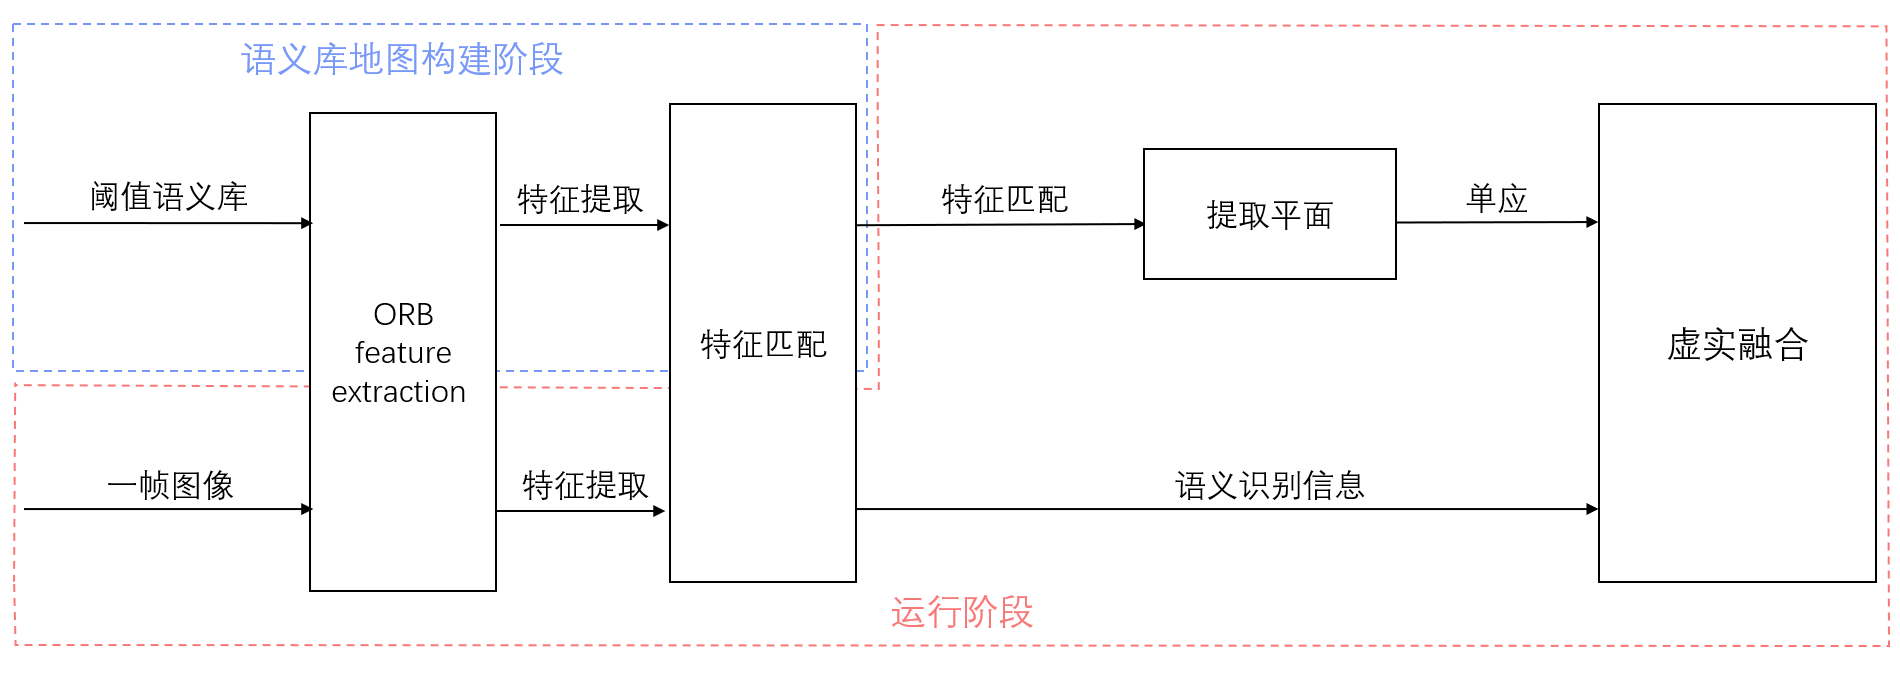
\includegraphics[width=0.5\textwidth]{Img/4-ismar.png}
    \bicaption{基于预置语义库地图的增强现实系统工作流程。}{Workflow of augmented reality system based on preset semantic library map.}
    \label{fig:ismar}
\end{figure}
对于一个已知的室外场景,我们预先取得其中标志性位置的图像,提取其中的特征点,构成预置语义库地图,因相比于SIFT或SURF,ORB特征点
能够达到实时的特征提取与匹配,同时具有较好的鲁棒性,因此,我们选择了ORB特征点构造预置语义库地图,表示为$\mathbb{M}=\left\{map_{0},...,map_{n}\right\}$,$map_{i}=\left[lng_{i},lat_{i},alt_{i},\mathbb{F}_{i}\right]$,
其中各项分别表示这一地图点的地理位置,包括经度、纬度和海拔,以及从这张图像中提取到的特征点集合。

在程序运行的过程中,系统实时通过设备内置的GPS获取当前的地理坐标,在$t$时刻表示为$cor_{t}=\left[lng_{t},lat_{t},alt_{t}\right]$,
同时,实时计算设备与$\mathbb{M}$各地图点的地理距离$dis_{ti}$,若与某一元素的距离小于一阈值$dis_{0}$,则认为当前设备进入了
此地图点的可视范围。

由于地图点可能分布较密集,其间距可能它小于GPS的精度,因此不能仅依靠以GPS坐标计算的设备与地图点的间距来识别地图点。在设备进入一
可是范围后,我们使用特征匹配的方法进行进一步精确的图像识别。具体来说,在进入一可视范围后,会对相机捕获的图像也提取ORB特征点,
与可视范围内的所有地图点存储的特征点集合进行匹配。对具有最高匹配相似度且高于一定阈值的地图点,认为当前设备所捕捉的图像正是
此地图点所存储的相应图像,系统可以从语义库中读取关于此位置的环境信息。

若连续两帧$F_{k-1}$、$F_{k}$匹配到了同一地图点,对这两帧图像的特征点$\mathbb{F}_{k-1}$、$\mathbb{F}_{k}$
,将仅保留与地图点特征点集相匹配的特征点,$\mathbb{F}_{k-1}^{'}$、$\mathbb{F}_{k}^{'}$,并对$\mathbb{F}_{k-1}^{'}$和$\mathbb{F}_{k}^{'}$
再次进行匹配,用匹配结果来计算对应环境平面的单应,得出相机坐标系到此地图点对应场景平面的转移矩阵。通过与地图点的特征匹配
保留下来的特征点,将是仅属于地图点对应场景平面的特征点,通过这些点之间的匹配关系计算的单应能够确保其唯一性,同时,因特征点数
的减少,程序运行开销也将降低。

具体的单应计算方法是,先通过RANSAC算法,从匹配点集中采用四个点对,计算单应矩阵初值$H_{0}$,之后通过最小化重投影误差,迭代
求得最优的单应:
$$H^{*}=\mathop{argmin}\limits_{H}\sum\limits_{i=1}^{n}\left \|f_{k}^{i}-Hf_{k-1}^{i} \right \|+\left \|f_{k-1}^{i}-H^{-1}f_{k}^{i} \right \|$$

根据以上方法,可以通过预先构造场景的预置语义库地图,通过结合GPS和特征识别的方法,识别设备所捕捉的图像并计算相机到场景平面的转移矩阵,获取对场景的语义理解。

\section{物体级语义地图的构建和表示}
\ref{cha_41}中介绍的基于局部特征的预置语义库地图需要预先构造语义库,仅能理解环境中少部分场景,没有在几何和语义层面对整个场景进行全面理解。SLAM系统
能够构造未知环境的几何地图,更好地全面理解并表示一个场景。然而传统基于特征的视觉SLAM系统构造的地图仅能表达几何空间结构,并且在
场景发生动态变化时会出现重影等问题。因此,本节研究了一种基于语义SLAM的物体级三维语义点云地图,能够结合对相机捕获的图像的实例级分割结果,
对其中物体分别建模并跟踪,为其赋予语义标签,并通过深度图像建立物体级的三维点云地图,给予场景高层的理解和表示。

\subsection{物体级语义点云地图生成方法}
在本文所提出的SLAM系统中,语义建图线程接受跟踪线程生成的关键帧$KF$和语义分割线程生成的关键帧的实例分割结果$\mathbb{R}$,
根据每一关键帧的信息增量式建图。语义建图线程处理一关键帧用时长于跟踪线程处理一帧的用时,为更好地利用计算资源,保证程序平滑运行,使得不同处理频率的线程同步进行,
我们创建了待处理关键帧队列$Q_{kf}$作为缓冲区,新生成的关键帧和相应的预测结果将插入$Q_{kf}$队尾,在处理过程中从将从队头取出。
\begin{figure}[!htbp]
    \centering
    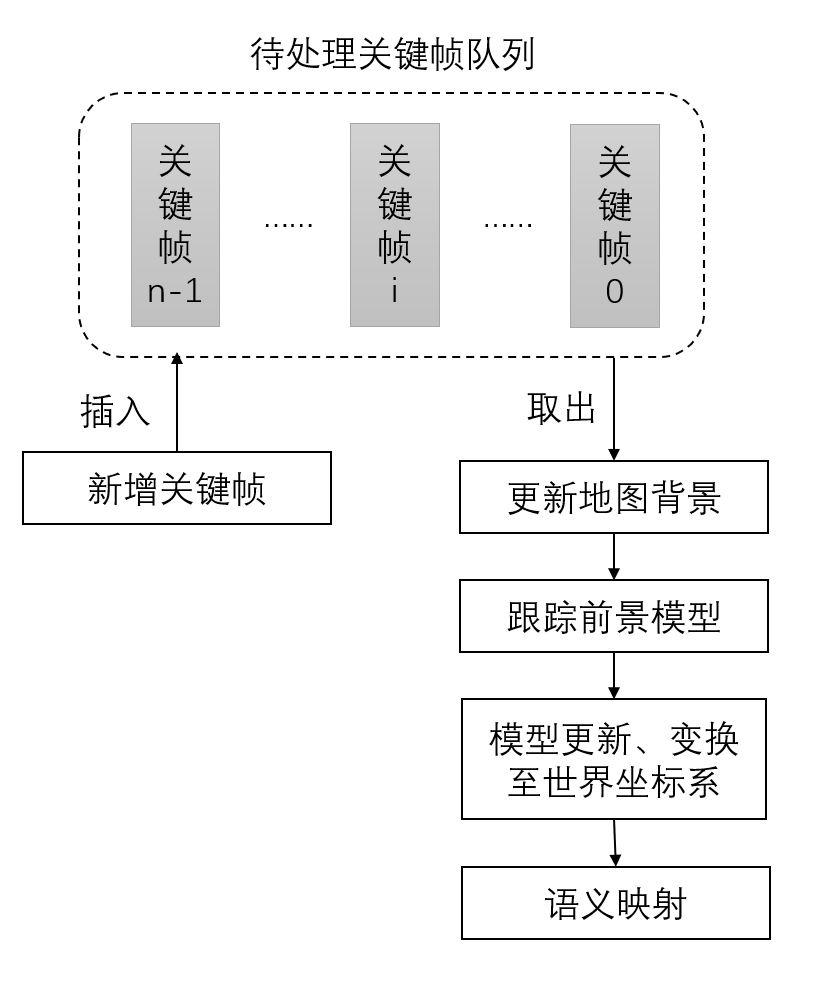
\includegraphics[width=\textwidth]{Img/4-queue.png}
    \bicaption{物体级语义建图模块工作流程。}{Object-level semantic mapping module workflow.}
    \label{fig:queue}
\end{figure}
本节研究的物体级语义地图由一个全局的背景模型$L_{0}$和一系列前景物体模型${L_{1},...,L_{i},...,L_{n}}$组成,前景物体模型将通过模型列表$\mathbb{L}$进行管理和维护。
其中$L_{i}=\left[\mathbb{PC}_{i}, cls_{i}, id_{i}, num_{i}, flag_{i} \right]$,各项表示此模型的点云模型、类别标签、模型编号、
连续跟踪丢失的帧数和成功跟踪标记。$\mathbb{PC}_{i}=\left[pc_{i}^{0},...,pc_{i}^{s},...,pc_{i}^{m}\right]$为一系列三维点集合,其中每个点表示为$pc_{i}^{s}=\left \{ x, y, z, b, g, r \right \}$,
分别为这一三维点在世界坐标系下的坐标和表示颜色的RGB分量。值得一提的是,对于全局背景模型$L_{0}$来说,它仅包含$\mathbb{PC}_{0}$和$id_{0}$两项。

建图过程中,系统增量式地更新$L_{0}$,为适应环境中目标的动态变化,会对$\mathbb{L}$中的模型进行跟踪,
为新检测到的物体建模、为跟踪到的物体模型更新、并删除跟踪丢失的模型。对每个关键帧完成模型跟踪后,将当前$\mathbb{L}$中可见的所有模型分别变换到
世界坐标系下的地图中,从而地图中物体模型随实现环境中物体移动而变化的效果。

下面以更新$L_{0}$为例,介绍增量式更新点云模型的方法。首先从$Q$队首取出关键帧$KF$和实例级分割结果$\mathbb{R}$,$KF$包括此帧的
彩色图$C$和深度图$D$。在$D$中,以一定步长间隔$step$取点,在实验中我们选取$step=3$,所取点$P=[u, v]$需满足:
\begin{equation} 
    \adddotsbeforeeqnnum%
    \begin{cases}
        m_{u,v}=0\\
        d_{min}<d<d_{max}\\
    \end{cases}
\end{equation}
即点$P$非前景目标,且深度值在一定范围内。其中$d=D(u,v)$,$d_{min}$和$d_{max}$为预设的深度阈值。

接下来通过相机内参$K$将$P$投影到相机坐标系下,得到点$X=[x,y,z]$:
\begin{equation} 
    \adddotsbeforeeqnnum%
    \begin{cases}
        x=\frac{u-cx}*d{fx}\\
        y=\frac{v-cy}*d{fy}\\
        z=d
    \end{cases}
\end{equation}

之后根据视觉里程计模块对此关键帧估计的位姿转移矩阵$T_{cw}$,将$X$变换至世界坐标系下,得到$\hat{X}$,即为对应点云模型中一点$pc$的
前三维分量。同时以彩色图上此点的r、g、b值$C(u,v)$作为$pc$的后三维分量:
\begin{equation} 
    \adddotsbeforeeqnnum%
    \begin{cases}
        pc_{0:2}=T_{cw}^{-1}\hat{X}\\
        pc_{3:5}=C(u,v)\\ 
    \end{cases}
\end{equation}

所有满足条件的点经处理后得到的三维点集合作为点云模型增量$L_{0}^{inv}$,用其更新$L_{0}$:
$$L_{0}=L_{0} \oplus L_{0}^{inv}$$
其中$\oplus$表示点云的融合相加操作。

前景模型的跟踪与之相似,不同之处为,对一个前景模型$L_{i}$和相应目标检测结果$r_{j}$,其选点需满足的条件为:
\begin{equation} 
    \adddotsbeforeeqnnum%
    \begin{cases}
        w_{m_{u,v}}=c_{j}\\
        d_{min}<d<d_{max}\\
        bu_{j}\geq u\geq bu_{j}+bw_{j}\\
        bv_{j}\geq v\geq bv_{j}+bh_{j}\\
    \end{cases}
\end{equation}
即点$P$为$r_{j}$的一前景点,且其深度在对应范围内。

此外,在生成三维点云时的步骤也有所不同,对于前景模型,将根据其类别$cls_{i}$选取对应颜色作为$pc$的后三维分量,点云地图
中各物体不同的颜色表示其不同的物体类别。

\subsection{物体建模和跟踪方法}

本研究的模型跟踪策略基于以下两个观察:
{
\setlist[enumerate]{}% restore default behavior
\begin{enumerate}[nosep]
    \item 对于一个运动中的物体,尤其是非刚体运动,比如人的挥手动作,增量式更新前景目标模型会导致形变局部产生重影。
    \item 对于静态的前景物体,其在连续关键帧之间的坐标位置不会有跳跃性的改变,而在局部遮挡、视野缺失等情况下容易跟踪失败。
\end{enumerate}
}
因此,我们提出了基于物体运动类别的模型跟踪策略。
对动态前景目标和静态前景目标,设置了不同的跟踪阈值$TT_moving$、$TT_static$和丢失阈值$TL_moving$、$TL_static$,
分别表示跟踪成功的最小IoU和跟踪丢失的最小连续帧数。
在程序运行阶段,对于检测到的一个物体$r_{j}$,首先根据其类别判定是否可能处于运动状态,若$w_{c_{j}}>0$,则认为此目标是一个
动态前景目标,反之认为此目标是一个静态前景目标,然后根据目标的运动类别选择相应的跟踪阈值和丢失阈值。一个模型的跟踪成功与否,
依靠当前关键帧检测到的个目标与其重合程度来计算,本研究使用了连续两关键帧上轮廓的IoU表示,IoU越大可能意味着此目标发生运动,或视野缺失。
对于动态前景目标,发生移动后应倾向于对其重新建模,以避免运动而产生的模型重影,因此其跟踪条件更为严格。
对于静态前景目标,发生移动后应倾向于对其进行维护,以避免因视野确实而造成的跟踪丢失,因此其跟踪条件更为宽松。

我们保存了上一个关键帧的语义mask$m_{pre}$和检测结果$\mathbb{R}_{pre}$,
对于当前关键帧检测到的目标,在跟踪过程中使用$\mathbb{L}$中同类别模型的语义mask和当前目标的语义mask计算IoU,根据IoU判定与模型的相似度。
直接在语义分割模块预测得到的2D语义mask上计算IoU,能够避免将模型投影到当前关键帧带来的大量计算开销。
而根据运动状态选择不同跟踪判断阈值,也能弥补相机视角变化带来的误差,从而使得跟踪过程具有较高的鲁棒性和准确度。

程序运行过程中,对于一个目标检测结果$r_{j}$,首先获取$\mathbb{L}$中与其同类别且未被跟踪到的模型集合$\mathbb{L}_{j}$,若此集合为空,
则为$r_{j}$新建一个模型插入模型列表,否则,使用$\mathbb{L}_{j}$的中模型依次与$r_{j}$计算IoU,得到最大的IoU和对应模型$MaxIoU, MaxL$。
之后,根据$MaxL$的先验权重$w_{cls_{MaxL}}$,判断其为动态前景目标还是静态前景目标,获取其对应的跟踪阈值$TT_{MaxL}$,若$MaxIoU$大于$TT_{MaxL}$,
则认为$MaxL$与$r_{j}$相匹配,跟踪成功,根据$r_{j}$计算点云模型增量,用以更新$\mathbb{PC}_{MaxL}$,更新此模型的连续跟踪失败帧数$num_{MaxL}$为0,设置跟踪成功标记$flag_{MaxL}$为真。否则,为$r_{j}$新建一个模型插入模型列表。
处理完所有检测到的目标的后,遍历$\mathbb{L}$中所有模型$L_{i}$,对于跟踪成功标记为假的模型,将其连续跟踪失败帧数加一。
之后,再次遍历$\mathbb{L}$中所有模型$L_{i}$,根据$MaxL$的先验权重$w_{cls_{i}}$,判断其为动态前景目标还是静态前景目标,获取其对应的丢失阈值$TL_{i}$,
若该模型的连续跟踪失败帧数$num_{i}$大于$TL_{i}$,则认为此模型跟丢,从模型列表中删除。

此算法具体描述为:
\begin{algorithm} %算法开始 
    \small
    \caption{模型跟踪算法} \label{alg1} %算法的标签 
    \begin{algorithmic}[1] %此处的[1]控制一下算法中的每句前面都有标号 
    \Procedure{跟踪后的模型列表}{$L^{'}$}
    \For{each $r_{j}$ in $\mathbb{R}$}
        \State $\mathbb{L}_{j}\gets GetModelInSameCategory(\mathbb{L},c_{j})$
        \If{$\mathbb{L}_{j}$ is empty}
            \State $L^{'}\gets BuildNewModel(r_{j})$
        \Else
            \For{each $L_{i}$ in $\mathbb{L}_{j}$}
                \State $IoU_{i,j}\gets CalIoU(m_{pre},\mathbb{R}_{pre},m,r_{j})$
                \State $MaxIoU, MaxL\gets UpdateClosestModel(IoU_{i,j},L_{i},MaxIoU, MaxL)$
            \EndFor
            \State $TT_{MaxL}\gets GetIoUThreshold(w_{cls_{MaxL}},TT_moving、TT_static)$
            \If{$MaxIou>TT_{MaxL}$}
                \State $L^{'}\gets UpdateModel(r_{j},MaxL)$
                \State $num_{MaxL}\gets 0$
                \State $flag_{MaxL}\gets true$
            \Else
                \State $L^{'}\gets BuildNewModel(r_{j})$
            \EndIf
        \EndIf
    \EndFor
    \For{each $L_{i}$ in $\mathbb{L}_{j}$}
        \If{$flag_{i} is false$}
            \State $num_{i}\gets num_{i}+1$
        \EndIf
    \EndFor
    \For{each $L_{i}$ in $\mathbb{L}_{j}$}
        \State $TL_{i}\gets GetLostThreshold(cls_{i},TL_moving、TL_static)$
        \If{$num_{i}>TL_{i}$}
            \State $L^{'}\gets DeleteModel(L_{i})$
        \EndIf
    \EndFor
    \EndProcedure
    \end{algorithmic} 
\end{algorithm}

\section{实验结果与分析}
我们使用TUM RGB-D数据集中高度动态的片段\emph{walking\_xyz}来测试了物体级语义地图的构建和表示效果。\ref{fig:maps}展示了在
第63帧和第87帧,原彩色图、深度图、实例分割结果和物体级语义建图结果图。可以看出,经实例分割得出的前景目标都被单独建模显示在了
三维点云地图的正确中,并且被赋予了不同颜色,以表示其类别。这里,蓝色表示类别“人”,红色表示类别“显示器”,紫色表示类别“椅子”,
黄色表示类别“水杯”。此外,在第63帧和第87帧直接,场景中人物发生了移动,而三维地图中对应模型也进行了相应更新。

\begin{figure}[!htbp]
    \centering
    \begin{subfigure}[b]{0.35\textwidth}
      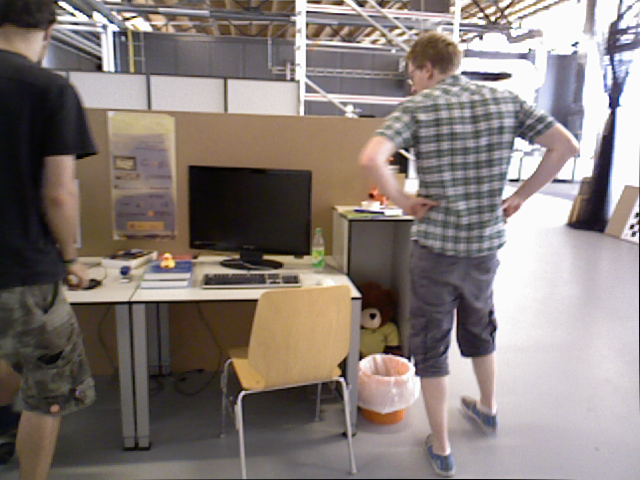
\includegraphics[width=\textwidth]{Img/ori_63.png}
      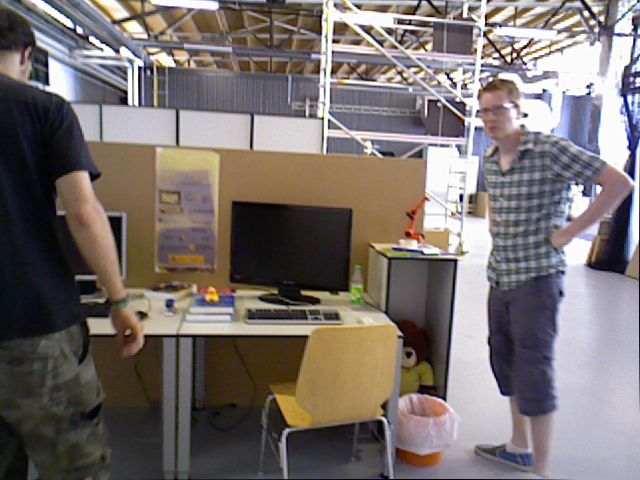
\includegraphics[width=\textwidth]{Img/ori_87.png}
      \caption{}
      \label{fig:ori}
    \end{subfigure}%
    \begin{subfigure}[b]{0.35\textwidth}
      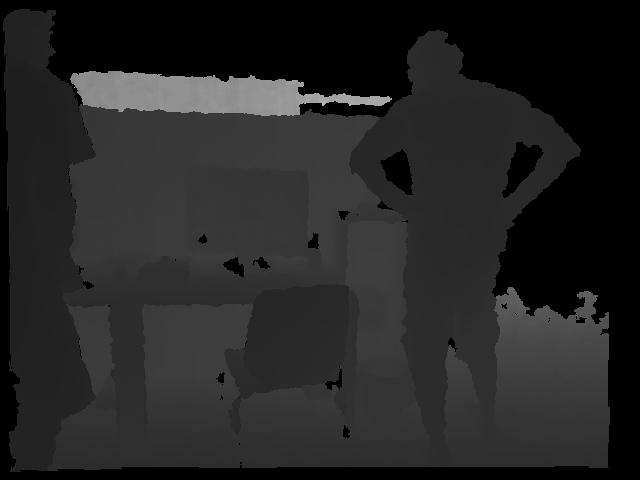
\includegraphics[width=\textwidth]{Img/depth_63.png}
      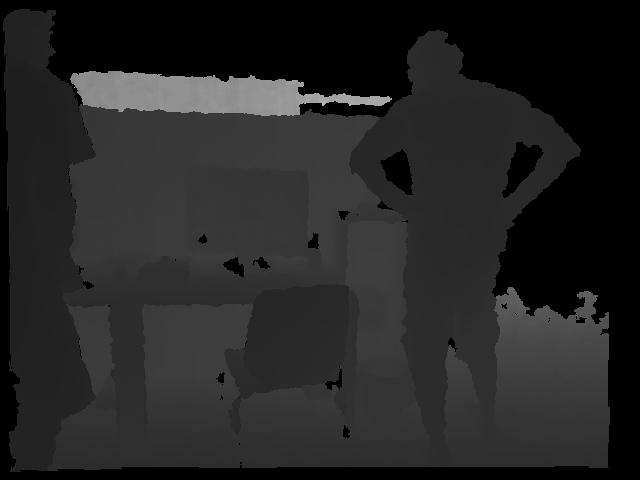
\includegraphics[width=\textwidth]{Img/depth_63.png}
      \caption{}
      \label{fig:depth}
    \end{subfigure}%
    ~% add desired spacing
    \\% line break
    \begin{subfigure}[b]{0.35\textwidth}
        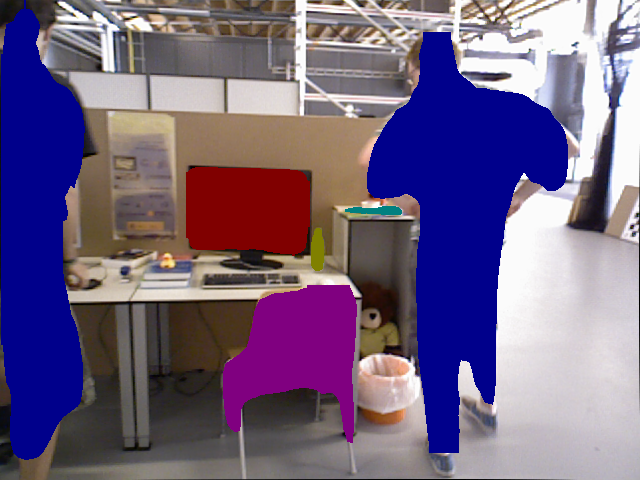
\includegraphics[width=\textwidth]{Img/mask_63.png}
        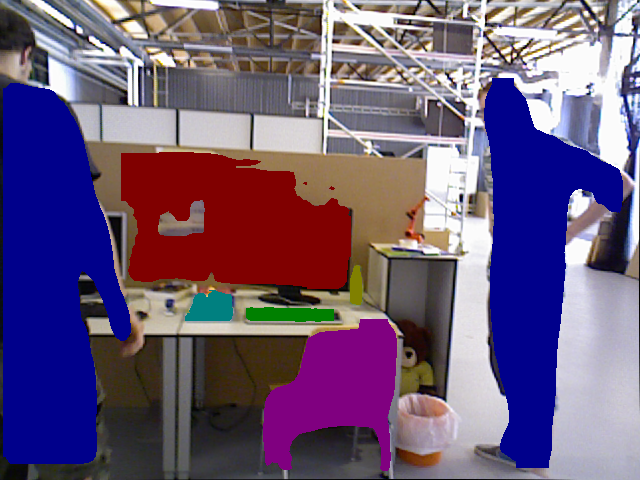
\includegraphics[width=\textwidth]{Img/mask_87.png}
      \caption{}
      \label{fig:mask}
    \end{subfigure}%
    ~% add desired spacing
    \begin{subfigure}[b]{0.35\textwidth}
        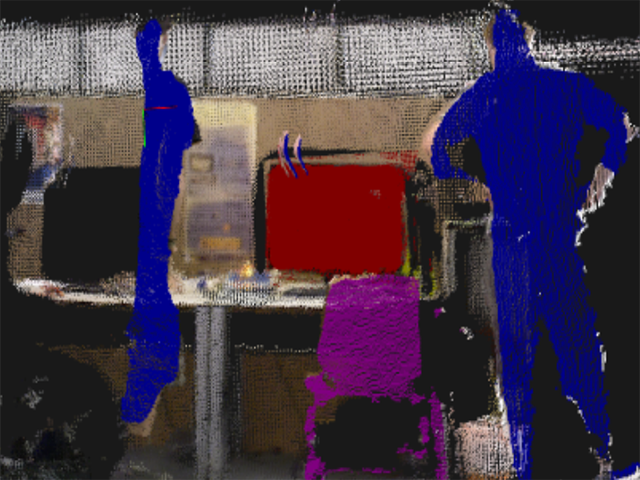
\includegraphics[width=\textwidth]{Img/map_63.png}
        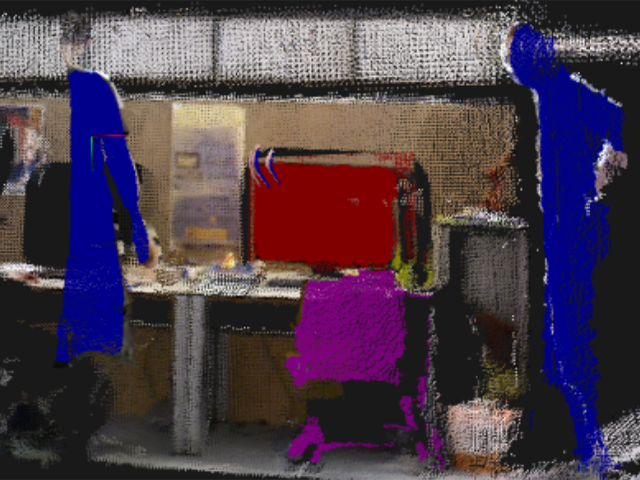
\includegraphics[width=\textwidth]{Img/map_87.png}
      \caption{}
      \label{fig:map}
    \end{subfigure}
    \bicaption{\emph{walking\_xyz}序列第63帧和第87帧的建图效果。(a) 原彩色图,(b) 原深度图,(c) 实例分割结果,(c) 物体级语义建图效果。}{ Illustration of our experimental results for frame 63 and frame 87 in sequence \emph{walking\_xyz}. 
    (a) the raw RGB image, (a) the raw depth image, (c)instance-level segmentation results, (c)object-aware semantic point cloud map.}
    \label{fig:maps}
\end{figure}
  
然而当前物体级语义地图构建和表示方法仍存在一些问题,比如地图中物体边缘不够精准,存在比较多的黑色孔洞等,需要在之后的工作中完善。

\section{本章小结}
本章按照不同的语义表达方式,讨论了两种语义地图的构建和表示方法。首先介绍了基于局部特征的预置语义库地图的构建和表示方法,
之后介绍了基于语义SLAM的物体级三维语义点云地图的构建和表示方法。这二者分别侧重于室外场景和动态场景,都能够一定程度上对于环境在语义层面上进行表达,从而用于增强显示应用的虚实融合方法优化。
在基于语义SLAM的物体级三维语义点云地图的构建方面,本章还详述了其在动态环境根据目标类别而指定物体跟踪策略。
最后给出了物体级三维语义点云地图的建图效果图,对实验结果进行了分析。